% Intended LaTeX compiler: pdflatex
\documentclass[10pt,a4paper,UTF8]{article}
\usepackage{zclorg}
\author{emacsun}
\date{}
\title{曲线拟合之概率回访}
\hypersetup{
 pdfauthor={emacsun},
 pdftitle={曲线拟合之概率回访},
 pdfkeywords={},
 pdfsubject={},
 pdfcreator={Emacs 25.0.50.1 (Org mode 9.0.5)},
 pdflang={English}}
\begin{document}

\maketitle
\tableofcontents
\titlepic{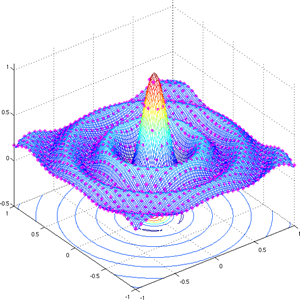
\includegraphics[scale=0.25]{../../img/sinc.PNG}}

\section{回忆}
\label{sec:orgd226b53}


我们之前在 \href{PRMLch1dot1-polynomial-curve.org}{曲线拟合的过程中} 采用的是最小化误差函数的方法来确定拟合的\(\mathbf{w}\)系数。拟合的多项式为:
\begin{equation}
\label{eq:1}
y(x, \mathbf{w}) = w_{0} + w_{1}x + \ldots + w_{M}x^{M} = \sum_{j=0}^{M}w_{j}x^{j}
\end{equation}

误差函数为:
\begin{equation}
\label{eq:2}
E( \mathbf{w}) = \frac{1}{2} \sum_{n=1}^{N}\{y(x_{n}, \mathbf{w}) - t_{n}\}^{2}
\end{equation}
在那里,我们为了解决过度拟合问题还采用了一种叫做正则化的方法。今天,我们从概率的角度来审视多项式曲线拟合问题。通过概率角度,我们可以更深入的理解误差函数和正则化。

\section{贝叶斯估计}
\label{sec:org88c1826}


曲线拟合的目的是对于给定输入\(x\)估计输出\(t\)。当然,我们有训练数据:对于\(\mathbf{x}= (x_{1},\ldots ,x_{N})^{T}\),对应的值是\(\mathbf{t} = (t_{1},\ldots ,t_{N})^{T}\)。对于任意的新的输入值\(x\),我们可以把对\(t\)的估计写成一个条件概率估计。什么样的概率密度函数最合适呢?\href{file://c:/Users/cliyh/AppData/Roaming/zorg/output/math/probability/afcp-normal-distribution-history.org}{正态分布最合适} !即,对于给定的输入\(x\),我们假设\(t\)具有正态分布,均值是\(y(x, \mathbf{w})\):
\begin{equation}
\label{eq:3}
p(t|x, \mathbf{w}, \beta) = \mathcal{N} (t| y(x, \mathbf{w}), \beta^{-1})
\end{equation}
其中\(\beta\)是精度参数,等于(\ref{eq:3})的方差的导数,即\(\beta^{-1} = \sigma^{2}\)。

式(\ref{eq:3})的示意图如\ref{fig:org99f83d0}所示。
\begin{figure}[htbp]
\centering
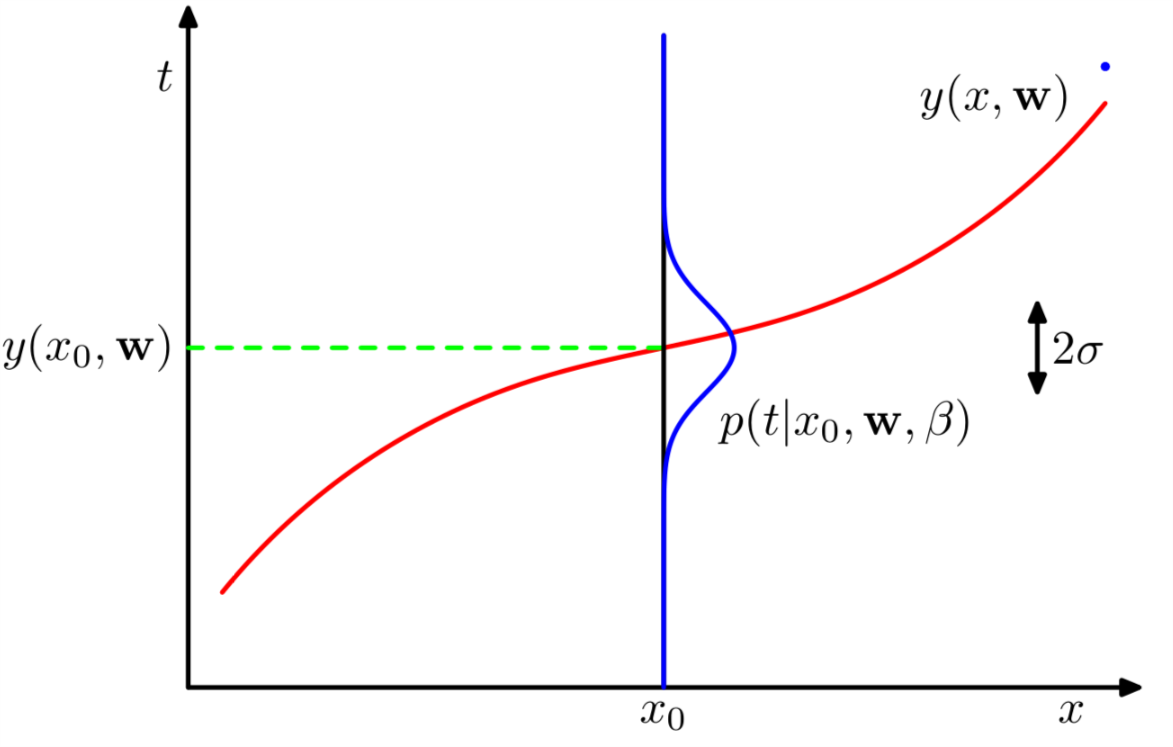
\includegraphics[width=0.6\textwidth]{../../img/computer_prml/20170502figure1dot16.png}
\caption{\label{fig:org99f83d0}
式(\ref{eq:3})的示意图}
\end{figure}

从图\ref{fig:org99f83d0} 中可以看出蓝色曲线就是假设的高斯分布。而精度值\(\beta\)体现了分布的方差。

现在我们用不同于 \href{PRMLch1dot1-polynomial-curve.org}{以往} 的方法来求\(\mathbf{w},\beta\)。如果所有的训练数据都是从(\ref{eq:3}) 中独立获得的,也就是说假设\(\mathbf{t}\)是独立同分布的。那么关于\(\mathbf{t},\mathbf{x}\)分布的似然函数是:
\begin{equation}
\label{eq:4}
p( \mathbf{t} | \mathbf{x}, \mathbf{w},\beta) = \prod_{n=1}^{N} \mathcal{N}(t_{n}|y(x_{n}, \mathbf{w}) \beta^{-1} )
\end{equation}

其中:
\begin{equation}
\label{eq:5}
\mathcal{N} (y| \mu, \sigma^{2} ) = \frac{1}{\sqrt{2\pi \sigma^{2}}} e^{-\frac{(x-\mu)^{2}}{2\sigma^{2}}}
\end{equation}

把(\ref{eq:5})带入(\ref{eq:4}),并对(\ref{eq:4})左右两端取自然对数:
\begin{equation}
\label{eq:6}
\ln p( \mathbf{t} | \mathbf{x}, \mathbf{w}, \beta) = -\frac{\beta}{2}\sum_{n=1}^{N}(y(x_{n}, \mathbf{w}) - t_{n})^{2} + \frac{N}{2}\ln \beta - \frac{N}{2}\ln(2\pi)
\end{equation}
我们从(\ref{eq:6})推出曲线拟合系数\(\mathbf{w}\)的最大似然解。显然,我们可以忽略(\ref{eq:6})的后两项,因为这两项与\(\mathbf{w}\)没有关系。另外我们也发现\(\mathbf{w}\)的最大似然解与等号右边第一项的系数也没有关系,这个系数只是起到缩放作用,我们还可以把\(\beta/2\)用\(1/2\)代替。最大化似然函数等效于最小化负的似然函数。最后我们发现最大化(\ref{eq:6})和最小化(\ref{eq:2})是一回事儿。 \textbf{因此(\ref{eq:2})所示的误差函数最小值的解是假定噪声为高斯噪声的最大似然解。}

另外我们还可以使用最大似然准则求得精度值\(\beta\)的最优解。把(\ref{eq:6})当做\(\beta\)的函数,我们有\(\beta\)的最大似然解满足:
\begin{equation}
\label{eq:7}
\frac{1}{\beta_{ML}} = \frac{1}{N}\sum_{n=1}^{N} \sum_{n=1}^{N}(y(x_{n}, \mathbf{w}) - t_{n})^{2}
\end{equation}

所以我们可以先求得\(\mathbf{w}\)的最大似然解\(\mathbf{w_{ML}}\),然后求得\(\frac{1}{\beta_{ML}}\)。如此,我们便得到了所需高斯分布的两个重要参数,对于任意输入\(x\),我们可以使用这个模型来估计\(t\)。
\section{概率模型}
\label{sec:orgdc673e7}


现在我们有了\(\mathbf{w}_{ML}\),\(\frac{1}{\beta_{ML}}\),我们就有了一个概率模型:
\begin{equation}
\label{eq:8}
p(t|x, \mathbf{w}_{ML}, \beta_{ML}) = \mathcal{N}(t| y(x, \mathbf{w}_{ML}), \beta_{ML}^{-1} )
\end{equation}

对于给定的\(x\)我们用(\ref{eq:1})来计算其均值\(y(x, \mathbf{w}_{ML})\),然后用(\ref{eq:8})给出\(t\)的估计。

现在让我们更深入的理解这个问题。首先,我们引入对(\ref{eq:1})中系数\(\mathbf{w}\)的一个先验估计:
\begin{equation}
\label{eq:9}
p( \mathbf{w} | \alpha) = \mathcal{N}( \mathbf{w} | \mathbf{0}, \alpha^{-1} \mathbf{I}) = (\frac{ \alpha}{ 2\pi})^{(M+1)/2} \exp(-\frac{\alpha}{2} \mathbf{w}^{T} \mathbf{w})
\end{equation}
其中\(\alpha\)是先验概率分布的精度。\(M+1\)是\(M\)阶多项式中的系数个数。\(\alpha\)控制着模型的参数(式(\ref{eq:1})的参数),我们称\(\alpha\)为超参数。据贝叶斯理论\(\mathbf{w}\)的后验分布与先验分布和似然函数成比例,即:
\begin{equation}
\label{eq:10}
p(\mathbf{w} | \mathbf{x},\mathbf{t}, \alpha,\beta) \propto p( \mathbf{t} | \mathbf{x}, \mathbf{w},\beta)p( \mathbf{w} | \alpha)
\end{equation}

利用给定的训练数据,我们通过最大化后验概率来确定\(\mathbf{w}\)。这个准则叫做最大后验概率准则(maximum posterior, MAP).  结合(\ref{eq:10})(\ref{eq:6})(\ref{eq:9}),我们发现最大后验概率等效于最小化(\ref{eq:11}):
\begin{equation}
\label{eq:11}
\frac{\beta}{2}\sum_{n=1}^{N} (y(x_{n}, \mathbf{w}) - t_{n} )^{2} + \frac{\alpha}{2} \mathbf{w}^{T} \mathbf{w}
\end{equation}

即,最大化后验概率等效于最小化带有正则参数\(\lambda = \alpha/\beta\)的均方误差函数。

\section{我们离真正的贝叶斯估计有多远}
\label{sec:org4e00da5}


截止目前,尽管我们引入了\(\mathbf{w}\)的一个先验估计\(p(\mathbf{w}|\alpha)\),但是我们还是在做\(\mathbf{w}\)的点估计,算不得真正的贝叶斯方法。因为“纯真血统”的贝叶斯方法需要一直使用概率的和积准则。这个和积准则的实用牵涉到边缘概率的计算。而边缘概率的计算是使用贝叶斯方法进行模式识别的核心内容。

在曲线拟合问题中,给定了训练数据\(\mathbf{x}, \mathbf{t}\),还有一个测试点\(x\),我们的目标是估计\(t\)。因此,我们希望对\(p(t|x, \mathbf{w}, \mathbf{t})\)做一个评估。

贝叶斯估计求解\(p(t|x, \mathbf{w}, \mathbf{t})\)的过程应该是:
\begin{equation}
\label{eq:12}
p(t| x, \mathbf{x}, \mathbf{t}) = \int p(t | x, \mathbf{w})p( \mathbf{w} | \mathbf{x}, \mathbf{t}) \mathrm{d} \mathbf{w}
\end{equation}
式 (\ref{eq:12}) 中\(p(t| x, \mathbf{w})\)由 (\ref{eq:3})给出。此处,我们准备忽略\(\alpha, \beta\)来简化符号表示。 \(p( \mathbf{w} | \mathbf{x}, \mathbf{t})\)是 参数\(\mathbf{w}\)的后验概率,可以对 (\ref{eq:10})归一化获得。稍后我们会发现,对于曲线拟合问题,这个后验概率分布是高斯分布,进而式 (\ref{eq:12})可以推演成:
\begin{equation}
\label{eq:13}
p(t| x, \mathbf{x}, \mathbf{t}) = \mathcal{N}(t| m(x), s^{2}(x))
\end{equation}

其中均值和方差为:
\begin{eqnarray}
\label{eq:14}
m(x) &=& \beta \mathbf{\phi}(x)^{T} \mathbf{S} \sum_{n=1}^{N}\mathbf{\phi}(x_{n})t_{n} \\
s^{2}(x) &=& \beta^{-1} + \mathbf{\phi}(x)^{T} \mathbf{S} \mathbf{\phi}(x)
\end{eqnarray}
矩阵\(\mathbf{S}\)为:

\begin{equation}
\label{eq:15}
\mathbf{S}^{-1} = \alpha \mathbf{I} + \beta\sum_{n=1}^{N} \mathbf{\phi}(x_{n}) \mathbf{\phi}(x)^{T}
\end{equation}
其中\(\mathbf{I}\)是单位阵。\(\mathbf{\phi}(x) = [\phi_{0}(x), \ldots ,\phi_{M}(x)], \phi_{i}(x) = x^{i}\)
我们看到式 (\ref{eq:14})所示的均值和方差依赖于\(x\)。方差的第一项\(\beta^{-1}\)代表了\(t\)的不确定度,这个不确定度是由噪声引起的。方差的第二项代表由\(\mathbf{w}\)带来的不确定度,这个不确定度是由贝叶斯方法带来的。
\end{document}
